\begin{figure}
    \centering
    \begin{subfigure}[t]{0.33\columnwidth}
        \centering
        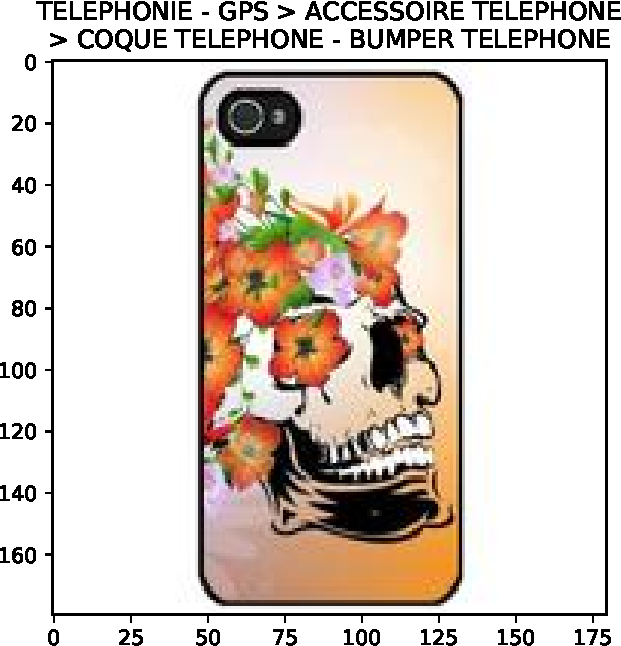
\includegraphics[width=\textwidth]{img/img-0-0}
        \caption{}
    \end{subfigure}%
    ~ 
    \begin{subfigure}[t]{0.33\columnwidth}
        \centering
        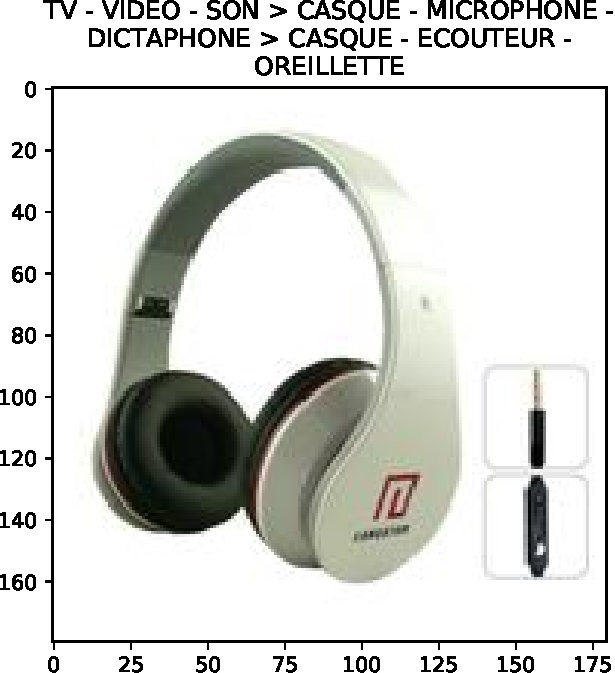
\includegraphics[width=\textwidth]{img/img-12-0}
        \caption{}
    \end{subfigure}%
    ~ 
    \begin{subfigure}[t]{0.33\columnwidth}
        \centering
        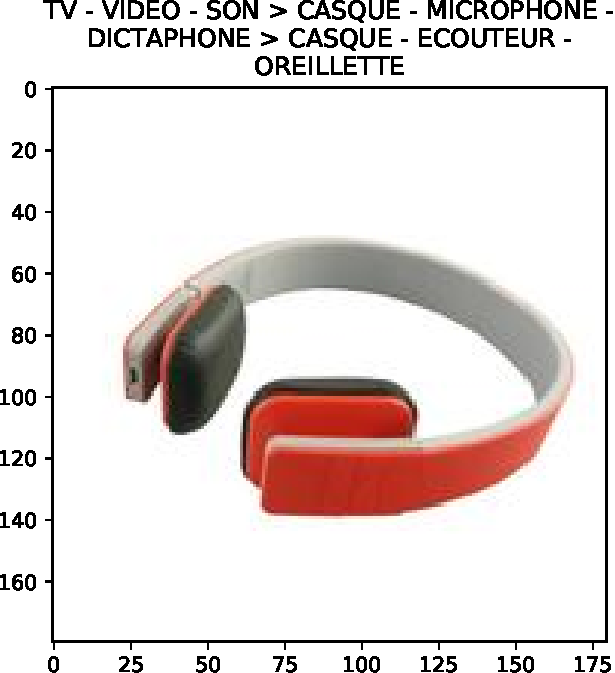
\includegraphics[width=\textwidth]{img/img-12-1}
        \caption{}
    \end{subfigure}
	\caption{
Images (a), (b), and (c) are three example training examples.
Image (a) is from a top level category different from images (b) and (c) (and therefore from different second and third categories, as well).
Images (b) and (c) are of the same product, and therefore from the same first, second, and third level categories.
Only some products, not all, have more than one associated image.
}
	\label{fig:example-images}
\end{figure}